\section{Auswertung}
\label{sec:Auswertung}
\subsection{Messung bei einem Druck unter $1\si{\bar}$}
In der Tabelle \ref{tab:p<1} sind die gemessenen Werte
von der Temperatur des Gases und der Druck
von der ersten Messung, die mit dem Versuchaufbau aus
dem Kapitel \ref{sec:p<1} durchgeführt wurde, aufgetragen.


\begin{table}  %Tabelle 1.Messung
  \centering
  \caption{Messwerte die mit Hilfe des Gerätes aus der Abbildung \ref{abb:p<1} gemessen wurden, bei einem Druch unter $1\,\si{\bar}$.}
  \label{tab:p<1}
  \begin{tabular}{c c}
    \toprule
    Temperatur des Gas &  Druck \\
    $T_\mathrm{g}/ \si{\kelvin}$ & $p/\si{\bar} $ \\
    \midrule
    307.15 & 0.080\\
    312.15 & 0.105\\
    320.15 & 0.132\\
    321.65 & 0.140\\
    323.65 & 0.150\\
    328.15 & 0.170\\
    330.15 & 0.180\\
    333.15 & 0.200\\
    338.15 & 0.250\\
    342.15 & 0.300\\
    346.15 & 0.350\\
    349.15 & 0.400\\
    352.15 & 0.450\\
    354.65 & 0.500\\
    357.15 & 0.550\\
    359.15 & 0.600\\
    361.15 & 0.650\\
    363.15 & 0.700\\
    365.15 & 0.750\\
    \bottomrule
  \end{tabular}
\end{table}

Werden diese nun in der Form $\log p$ in Abhängigkeit von $T$ aufgeträgen,
lässt sich mit Hilfe der Linearen Regression eine Ausgleichsgrade bestimmen.
Dies ist in der Abbildung \ref{abb:plot1} dargestellt.
\begin{figure}
  \centering
  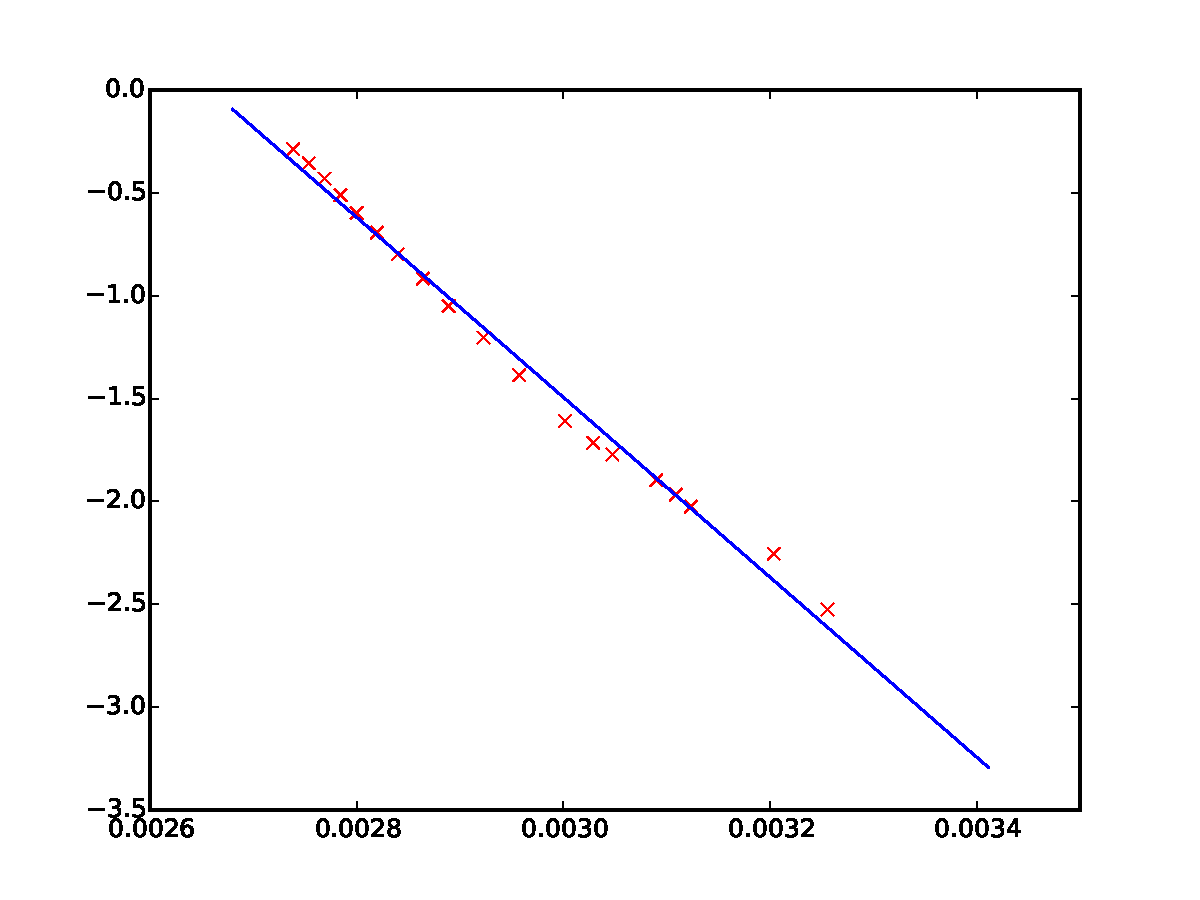
\includegraphics[width=0.7\textwidth]{plot1.pdf}
  \caption{Messwerte aus Tabelle \ref{tab:p<1} die in der Form $T_\mathrm{g}$ nach $\log p$ aufgetragen sind . }
  \label{abb:plot1}
\end{figure}
Aus der Linearen Regression ergibt sich für die Parameter:
\begin{align*}
  a=& -14,405\,\si{\bar}
  b=&   0,039\,\si{\bar\per\kelvin}
\end{align*}



\subsection{Messung bei einem Druck über $1\si{\bar}$}
Bei dieser Messung ergeben sich die in Tabelle \ref{tab:p>1} aufgelisteten Messwerte für $T_\mathrm{g}$ und $p$.
\begin{table}   % Tabelle 2.Messung
  \centering
  \caption{Messwerte die mit Hilfe des Gerätes aus der Abbildung \ref{abb:p>1} gemessen wurden, bei einem Druch über $1\,\si{\bar}$.}
  \label{tab:p>1}
  \begin{tabular}{c c}
    \toprule
    Temperatur des Gas &  Druck \\
    $T_\mathrm{g}/ \si{\kelvin}$ & $p/\si{\bar} $ \\
    \midrule
    295.15 & 1.00\\
    304.05 & 1.04\\
    316.45 & 1.12\\
    323.15 & 1.18\\
    333.15 & 1.29\\
    344.65 & 1.47\\
    353.15 & 1.65\\
    363.15 & 1.93\\
    373.15 & 2.32\\
    383.15 & 2.84\\
    393.15 & 3.51\\
    403.15 & 4.37\\
    413.15 & 5.47\\
    423.15 & 6.80\\
    433.95 & 8.63\\
    443.15 & 10.5\\
    453.15 & 13.0\\
    463.15 & 16.0\\
    472.15 & 19.4\\
    \bottomrule
  \end{tabular}
\end{table}
$p$ wird nun gegen $T_\mathrm{g}$ aufgetragen, wie in Abbildung \ref{abb:plot2} zusehen, und an die Messwerte wird ein Polynom
der Form
\begin{align*}
p(T)=a\cdot T^3+b\cdot T^2 + c\cdot T + d
\end{align*}
angenährt.
Die Konstanten des Polynoms werden mit scipy eine Erweiterung von Python ausgerechnet. Als Konstanten gegeben sich somit
\begin{align*}
  a =&0,0000058
  b =&-0,0057451
  c =&1,9074059
  d =&-210,6931553
\end{align*}
\begin{figure}
  \centering
  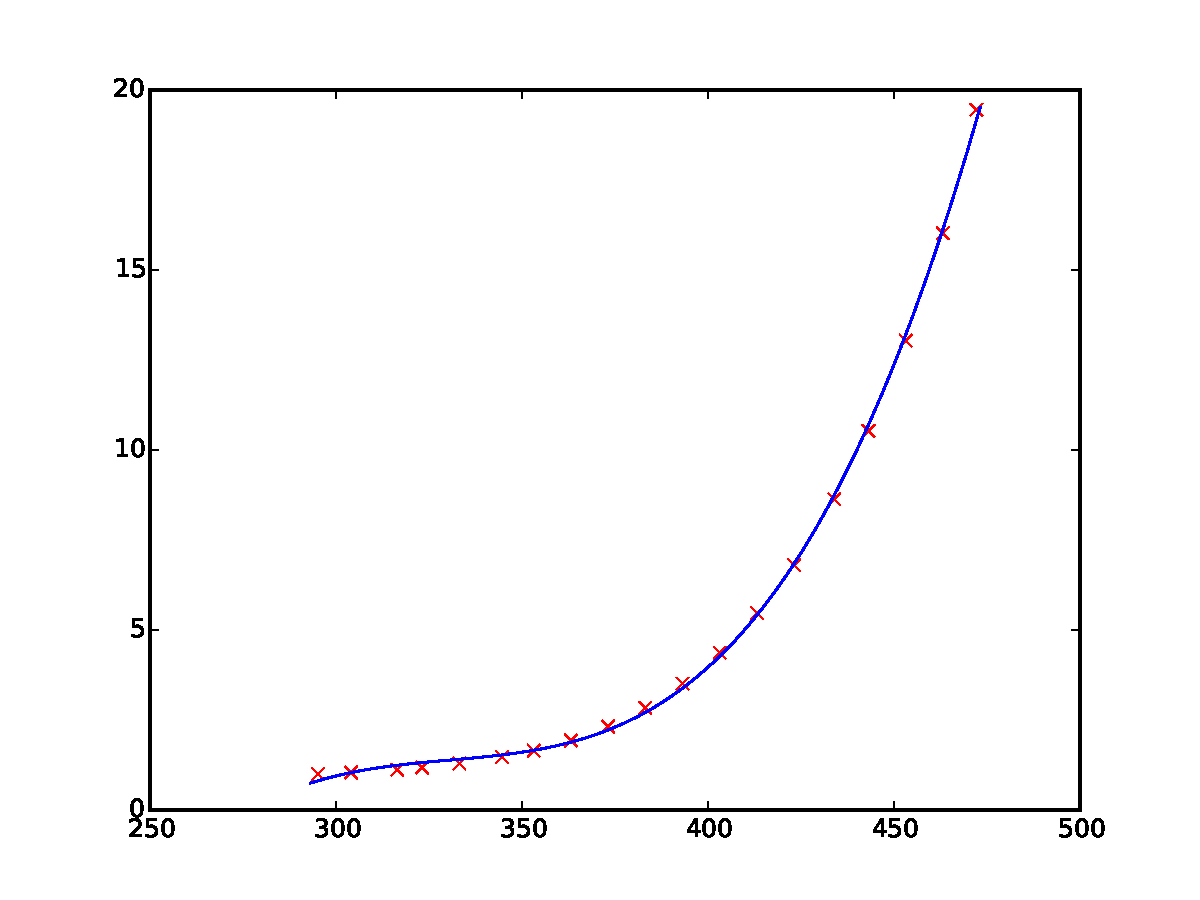
\includegraphics[width=0.7\textwidth]{plot2.pdf}
  \caption{Messwerte aus Tabelle \ref{tab:p>1} die in der Form $T_\mathrm{g}$ nach $p$ aufgetragen sind .}
  \label{abb:plot2}
\end{figure}





\begin{figure}
  \centering
  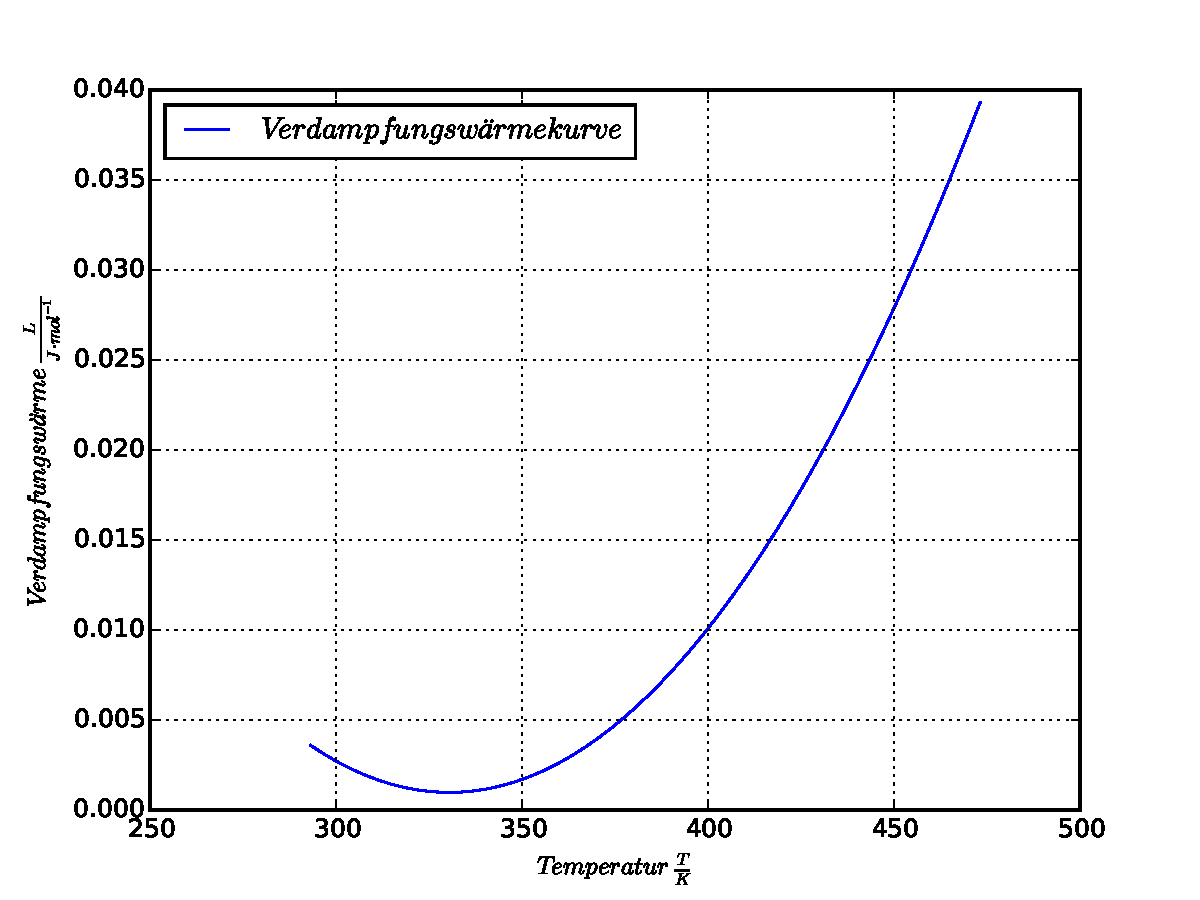
\includegraphics[width=0.7\textwidth]{plot3.pdf}
  \caption{Verdampfungswärme $L$ in Abhängigkeit von $T$ aus der Formel \eqref{eqn:-}.}
  \label{abb:graph-}
\end{figure}

\begin{figure}
  \centering
  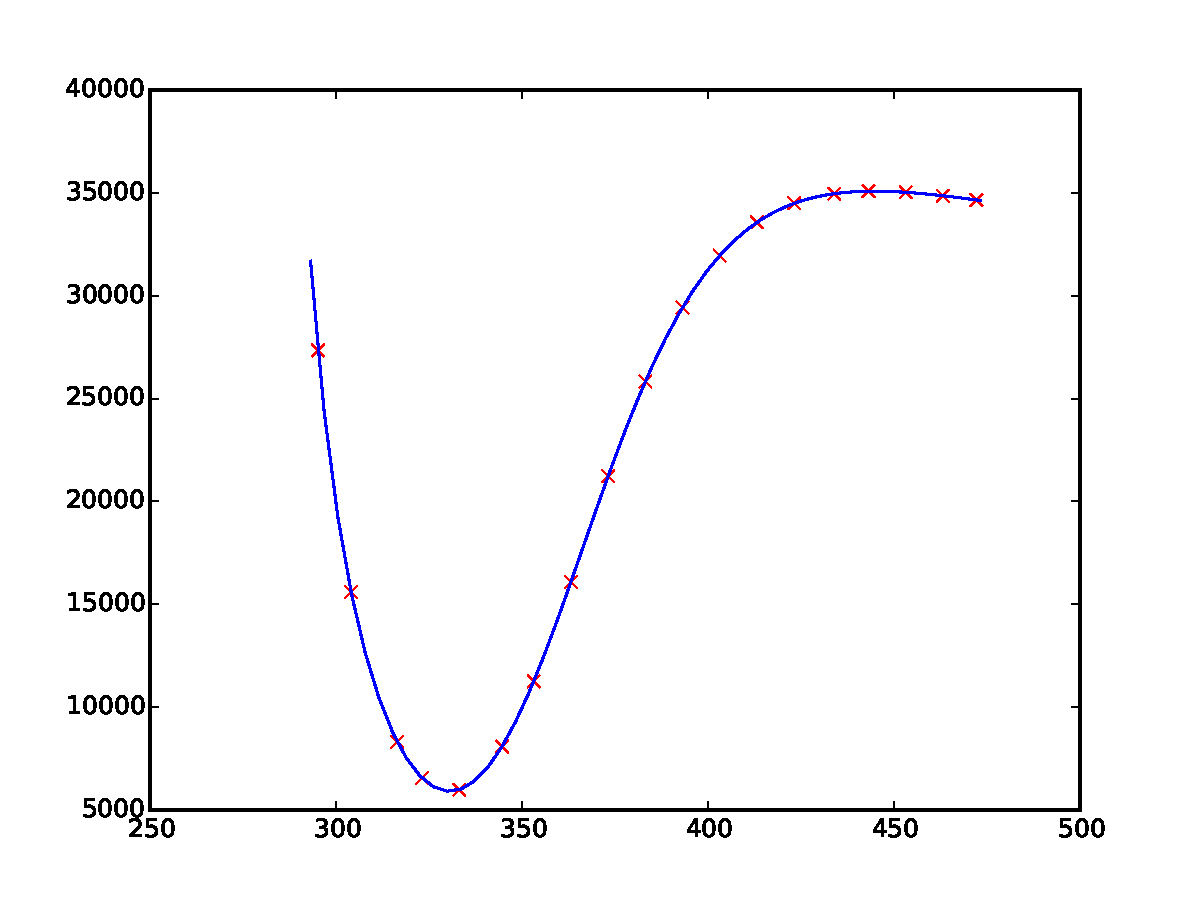
\includegraphics[width=0.7\textwidth]{plot4.pdf}
  \caption{Verdampfungswärme $L$ in Abhänigkeit von $T$ aus der Formel \eqref{eqn:+}.}
  \label{abb:graph+}
\end{figure}
